\documentclass[11pt]{article}
\usepackage[margin=1in]{geometry}
\usepackage[T1]{fontenc}
\usepackage{lmodern}
\usepackage{amsmath,amssymb,amsthm}
\usepackage{booktabs}
\usepackage{graphicx}
\usepackage{natbib}
\usepackage[hidelinks]{hyperref}
\usepackage{setspace}
\setstretch{1.15}

\newtheorem{theorem}{Theorem}
\newtheorem{proposition}{Proposition}
\newtheorem{lemma}{Lemma}
\newtheorem{corollary}{Corollary}
\theoremstyle{definition}
\newtheorem{definition}{Definition}
\newtheorem{assumption}{Assumption}
\theoremstyle{remark}
\newtheorem{remark}{Remark}

\newcommand{\E}{\mathbb{E}}
\renewcommand{\P}{\mathbb{P}}
\newcommand{\R}{\mathbb{R}}
\newcommand{\one}{\mathbf{1}}
\newcommand{\ip}[2]{\langle #1,#2\rangle}

\title{Two end modes: logarithmic asymptotics and importance sampling for the peak
load of a pickup-and-delivery route}
\author{Quang-Vinh Dang\\
British University Vietnam, Hung Yen, Vietnam\\
\texttt{vinh.dq4@buv.edu.vn}\quad ORCID 0000-0002-3877-8024}
\date{}

\begin{document}
\maketitle

\begin{abstract}
A vehicle that delivers and collects goods along a route of $L$ stops carries, after
stop $k$, the deliveries still to be made plus the pickups already made. We study the
probability that the peak of this load exceeds a large level $c$ when the demands are
gamma variables coupled by one-factor Gaussian copulas, one for deliveries and one for
pickups. The peak is a maximum of $L+1$ sums of transformed correlated normals, and
we show that $\log\P(\text{peak}>c) = -c/\lambda^\star + O(\sqrt c)$, where
$\lambda^\star$ is the larger of two explicit spectral scales: the largest root of a
secular equation for the delivery block at the start of the route and for the pickup
block at its end. Importance sampling with a single mean shift at the dominant end is
logarithmically efficient when the weaker end scale is below $\lambda^\star/4$ and the
dominant block has a spectral gap, and is not efficient when it is above
$\lambda^\star/4$. In the second case the failure need not show: when the
sample size is small compared with the inverse probability of the weaker end mode, with
high probability no draw reaches it, and given that, the estimate has mean equal to the
probability minus that mode's mass while its sample variance stays small. A mixture of shifts at the
dominating points of the stage blocks, with a defensive component, is logarithmically
efficient under a covering condition that we reduce to a two-dimensional min--max
problem, with closed-form sufficient conditions. On 5\,920 routes of two regional plans
the condition holds, for constant weights, on every route at copula correlation $0.6$; numerical checks
against a quadrature reference confirm the predicted underestimation of the single
shift and the accuracy of the mixture down to $10^{-6}$.

\medskip\noindent\textbf{Keywords:} rare-event simulation; importance sampling;
logarithmic efficiency; large deviations; Gaussian copula; quadratic forms; vehicle
routing.
\end{abstract}

\section{Introduction}
\label{sec:intro}

A vehicle leaves a depot with the goods for $L$ customers and, at each stop, unloads
the delivery $d_i$ and loads the pickup $p_i$. After stop $k$ it carries
\[
L_k = \sum_{i>k} d_i + \sum_{i\le k} p_i ,\qquad k=0,\dots,L,
\]
and it overflows a capacity $c$ if the peak $F=\max_k L_k$ exceeds $c$. This is the
load profile of the vehicle routing problem with simultaneous pickup and delivery
\citep{Dethloff2001}. When the demands are random, planning models control
$\P(F>c)$ at moderate levels \citep{GendreauJabaliRei2016,GounarisWiesemannFloudas2013,
DinhFukasawaLuedtke2018,GhosalWiesemann2020}; medical, cold-chain and dangerous-goods
distribution ask for levels between $10^{-3}$ and $10^{-6}$, which must then be verified
by simulation, and at such levels crude Monte Carlo needs $1.96^2/(\varepsilon^2 p)$
draws for relative error $\varepsilon$.

The probabilistic question is the tail of a maximum of dependent sums. The load process
$(L_k)$ is not a random walk: its increments $p_k-d_k$ change sign, the first term
$D_k=\sum_{i>k}d_i$ decreases and the second $P_k=\sum_{i\le k}p_i$ increases along the
route, and the demands within each type are correlated. We take gamma marginals and a
one-factor Gaussian copula for each type, $d_i = G_{d,i}^{-1}(\Phi(Z_{d,i}))$ with
$Z_{d,i}=\sqrt\rho\,W_d+\sqrt{1-\rho}\,E_{d,i}$, and likewise for pickups with an
independent factor $W_p$. The gamma quantile of a normal score grows like
$\theta z^2/2$, so each $L_k$ is, to leading order, a positive part of a quadratic form
in the Gaussian inputs, and its tail is governed by the largest eigenvalue of a matrix
$\Theta^{1/2}C\Theta^{1/2}$ built from the gamma scales and the copula correlation
\citep[the same structure appears in delta--gamma approximations of portfolio losses,][]
{GlassermanHeidelbergerShahabuddin2000}.

\paragraph{Contributions.}
(i) Theorem~\ref{thm:ld}: for every stage,
$\log\P(L_k>c) = -c/\lambda_k + O(\sqrt c)$ (with an $O(\log c)$ upper error), and
$\log\P(F>c) = -c/\lambda^\star + O(\sqrt c)$, where $\lambda_k$ is the larger of the
scales of the stage's delivery and pickup blocks, each the largest root of an explicit
secular equation, and $\lambda^\star = \max_k\lambda_k$ is attained, when $\rho>0$, only
at the two ends of the route (Corollary~\ref{cor:ends}). On the logarithmic scale a route overflows in
one of two \emph{end modes}: all deliveries on board at the start, or all pickups on
board at the end.

(ii) Theorem~\ref{thm:single}: let $\varrho\in(0,1]$ be the ratio of the weaker to the
stronger end scale. A single mean shift at the dominant end is not logarithmically
efficient when $\varrho>1/4$ (with a defensive component: when $\varrho>1/2$), and it
is logarithmically efficient when $\varrho\le1/4$ and the dominant end block has a
spectral gap of at least $4$.

(iii) Proposition~\ref{prop:silent}: in the inefficient case the second moment is
inflated by a region the proposal reaches only as often as crude Monte Carlo does. On the
event, of probability at least $1-N\,\P(\text{weaker end event})$, that no draw reaches
it, the estimate has conditional mean $p-\P(\text{weaker end event})$ up to a factor
$1+O(p)$; its own sample variance does not reveal the deficit. We show that this
predicts the bias measured on real routes, of the single shift and of a two-step
Glasserman--Li estimator.

(iv) Theorem~\ref{thm:mixture}: a mixture of mean shifts at the asymptotic dominating
points of the stage blocks, with weights that may decay like $e^{-c\delta_m}$ and a
defensive component, is logarithmically efficient when every stage satisfies a covering
inequality $\Psi_k\ge4\lambda_k/\lambda^\star$. The constant $\Psi_k$ is the value of a
two-dimensional min--max problem in the stage's spectral ratios; Lemma~\ref{lem:psi}
evaluates it in closed form in the cases that matter ($\Psi=4$ when one block of the stage
dominates the other by a factor $3$ and both have a spectral gap of $3$; $\Psi\ge2\sqrt2$
under a gap of $2$, with equality for a tie), and
Corollary~\ref{cor:plan} extends the result to several routes sharing the factors.

(v) Section~\ref{sec:numerics} checks the conditions on 5\,920 routes of plans for two
regions (Northern Vietnam and Guangdong) and compares the estimators with a
quadrature reference, crude Monte Carlo, cross-entropy, Glasserman--Li two-step
sampling, conditional Monte Carlo and subset simulation at levels $10^{-3}$ to
$10^{-6}$.

\paragraph{Relation to the literature.}
The ingredients are classical, and we use them as such. Exponential twisting at a
dominating point is efficient under a geometric condition on the rare set
\citep{SadowskyBucklew1990,Bucklew2004}; a single twist fails when the rare set can be
reached in several ways \citep{GlassermanWang1997}; mixtures of twists are instances of
the subsolution approach of \citet{DupuisWang2007}; mixtures over the events of a union
have a uniform variance bound when each event can be sampled exactly conditionally
\citep{OwenMaximovChertkov2019}; and for factor copulas \citet{GlassermanLi2005} combine a
factor shift with conditional twisting \citep[see also][]{BassambooJunejaZeevi2008}. Our
model is not covered by these results as stated: the rare set is a union of
\emph{non-convex} sets (positive parts of quadratic forms of a Gaussian vector, after a
gamma quantile transform), its components overlap through shared factors, and the
conditional sampling that the bound of \citeauthor{OwenMaximovChertkov2019} needs is not
available. What we add is the explicit form of the scales and modes for the
pickup-and-delivery peak, the $1/4$ threshold with its silent-bias mechanism, and a
covering constant that turns the efficiency of a stage mixture into a computable
condition. Surveys of the efficiency notions are \citet{AsmussenGlynn2007} and
\citet{Bucklew2004}.

\section{Model and spectral scales}
\label{sec:model}

\subsection{Model}
Let $u=(W_d,W_p,E_{d,1},\dots,E_{d,L},E_{p,1},\dots,E_{p,L})$ be a standard normal vector
in $\R^n$, $n=2L+2$, with density $\varphi$. For $\rho\in[0,1)$ put
\[
Z_{d,i}=\sqrt\rho\,W_d+\sqrt{1-\rho}\,E_{d,i},\qquad Z_{p,i}=\sqrt\rho\,W_p+\sqrt{1-\rho}\,E_{p,i},
\]
and $d_i=x_{d,i}(Z_{d,i})$, $p_i=x_{p,i}(Z_{p,i})$ with $x(z)=G^{-1}(\Phi(z))$ and $G$ a
gamma distribution function of shape $\kappa>0$ and scale $\theta>0$ (both may depend on
the customer and the type). Then each $d_i$ and $p_i$ is gamma, deliveries are
dependent through $W_d$, pickups through $W_p$, and deliveries and pickups are
independent. With $L_k$ and $F$ as in the introduction, the object of study is
\[
p(c)=\P(A_c),\qquad A_c=\{F>c\}=\bigcup_{k=0}^L\{L_k>c\}.
\]
Every customer with positive mean has a positive scale; customers with zero mean
delivery or pickup contribute nothing and are dropped from the corresponding sums.
To keep the notation light we assume all $2L$ scales positive.

\subsection{Blocks}
For a type $b\in\{d,p\}$ and a set $S\subseteq\{1,\dots,L\}$ let $B_S$ be the $|S|\times n$
matrix with $(B_Su)_i=Z_{b,i}$, $i\in S$; its entries are nonnegative, each row has unit
norm, and $B_SB_S^\top=C_S=\rho\one\one^\top+(1-\rho)I$. With
$\Theta_S=\mathrm{diag}(\theta_{b,i})_{i\in S}$ define the $n\times n$ matrix
$M_S=B_S^\top\Theta_SB_S$, the quadratic forms
\[
h_S(u)=\tfrac12\sum_{i\in S}\theta_{b,i}\,(Z_{b,i})_+^2\ \le\ \tfrac12u^\top M_Su ,
\]
and the scales $\lambda(S)\ge\mu(S)$, the two largest eigenvalues of
$K_S=\Theta_S^{1/2}C_S\Theta_S^{1/2}$ (with $\mu(S)=0$ if $|S|=1$ and
$\lambda(\emptyset)=\mu(\emptyset)=0$). The nonzero eigenvalues of $M_S$ and $K_S$
coincide, with multiplicities.

\begin{lemma}[Spectral facts]\label{lem:spectral}
Let $S\ne\emptyset$ and $\xi=\Theta_S^{1/2}\one$.
\begin{enumerate}
\item[(a)] If $\rho>0$, $\lambda(S)$ is the unique root in
$((1-\rho)\max_{S}\theta,\infty)$ of
$1=\rho\sum_{i\in S}\theta_i/(\lambda-(1-\rho)\theta_i)$.
\item[(b)] $\rho\sum_S\theta_i+(1-\rho)\min_S\theta\le\lambda(S)\le\rho\sum_S\theta_i+(1-\rho)\max_S\theta$
and $\mu(S)\le(1-\rho)\max_S\theta$.
\item[(c)] If $S\subsetneq S'$ (same type) and $\rho>0$, then $\lambda(S)<\lambda(S')$.
\item[(d)] Let $v\ge0$ be a unit Perron vector of $K_S$. Then $e_S=B_S^\top\Theta_S^{1/2}v/\sqrt{\lambda(S)}$
is a unit eigenvector of $M_S$ for $\lambda(S)$, $e_S\ge0$, and $\beta_S=B_Se_S\ge0$
satisfies $\sum_{i\in S}\theta_i\beta_{S,i}^2=\lambda(S)$; if $\rho>0$ then $\beta_S>0$.
\end{enumerate}
\end{lemma}

\begin{proof}
$K_S=(1-\rho)\Theta_S+\rho \xi\xi^\top$. (a) For $\lambda>(1-\rho)\max\theta$,
$\lambda I-K_S=(\lambda I-(1-\rho)\Theta_S)\big(I-\rho(\lambda I-(1-\rho)\Theta_S)^{-1}ss^\top\big)$,
which is singular iff $1=\rho \xi^\top(\lambda I-(1-\rho)\Theta_S)^{-1}\xi$, the stated
equation. Its right side decreases from $+\infty$ to $0$ on the interval, so there is
exactly one root there. By Weyl's inequalities for a rank-one update
\citep[Thm.~4.3.4]{HornJohnson2013}, $K_S$ has at most one eigenvalue above
$(1-\rho)\max\theta$; it has one, because for the coordinate vector $\epsilon_j$ of a
customer with the largest scale, $\epsilon_j^\top K_S\epsilon_j=\theta_j>(1-\rho)\theta_j$.
Hence that eigenvalue is $\lambda(S)$ and it is the root.
(b) The lower bound is the Rayleigh quotient at $\xi/|\xi|$; the upper bound
follows from $K_S\preceq(1-\rho)\max\theta\,I+\rho \xi\xi^\top$ and $|\xi|^2=\sum\theta_i$;
the bound on $\mu$ is Weyl's inequality for a rank-one update of $(1-\rho)\Theta_S$.
(c) With $f_S(\lambda)=\rho\sum_{i\in S}\theta_i/(\lambda-(1-\rho)\theta_i)$, $f_{S'}>f_S$ on
$((1-\rho)\max_{S'}\theta,\infty)$; at $\lambda=\lambda(S')$ this gives
$f_S(\lambda(S'))<1=f_S(\lambda(S))$, and $f_S$ is decreasing, so $\lambda(S')>\lambda(S)$.
(d) $M_Se_S=B_S^\top\Theta_S^{1/2}K_Sv/\sqrt{\lambda}=\lambda e_S$ and
$|e_S|^2=v^\top K_Sv/\lambda=1$; nonnegativity follows from $B_S\ge0$ and the
Perron--Frobenius theorem for the nonnegative matrix $K_S$. Further
$\beta_S=C_S\Theta_S^{1/2}v/\sqrt\lambda$, which is positive when $\rho>0$ because $C_S$ has
positive entries and $v\ne0$; and
$\sum\theta_i\beta_{S,i}^2=e_S^\top M_Se_S=\lambda$.
\end{proof}

\subsection{Stages and end modes}
Stage $k$ has the delivery block $S^d_k=\{k+1,\dots,L\}$ and the pickup block
$S^p_k=\{1,\dots,k\}$, with scales $\lambda^d_k=\lambda(S^d_k)$, $\lambda^p_k=\lambda(S^p_k)$
and second eigenvalues $\mu^d_k,\mu^p_k$. Put
\[
\lambda_k=\max(\lambda^d_k,\lambda^p_k),\qquad
\lambda^\star=\max_k\lambda_k=\max(\lambda^d_0,\lambda^p_L),\qquad
\varrho=\frac{\min(\lambda^d_0,\lambda^p_L)}{\lambda^\star}\in(0,1],
\]
the second equality by Lemma~\ref{lem:spectral}(c) (or, for $\rho=0$, by Cauchy
interlacing). The two blocks of a stage act on disjoint coordinates of $u$, so
\[
h_k(u)=h_{S^d_k}(u)+h_{S^p_k}(u)
\]
is the positive-part quadratic form of stage $k$, with block-diagonal matrix of largest
eigenvalue $\lambda_k$. For a stage we call the block attaining $\lambda_k$ the dominant
block $H$ (either one in case of a tie) and the other the weak block; we write
\[
\varrho_k=\frac{\min(\lambda^d_k,\lambda^p_k)}{\lambda_k},\qquad
\nu_k=\frac{\max(\mu^d_k,\mu^p_k)}{\lambda_k},\qquad r_k=\frac{\lambda_k}{\lambda^\star}.
\]

\section{Two lemmas}
\label{sec:lemmas}

\begin{lemma}[Gamma quantile of a normal score]\label{lem:quantile}
Let $x(z)=G^{-1}(\Phi(z))$ for a gamma law of shape $\kappa$ and scale $\theta$. Then
$x(z)=\theta z^2/2+\theta(2\kappa-1)\log z+O(1)$ as $z\to\infty$, and there is a constant
$C$ such that
\[
x(z)\le\tfrac12\theta z_+^2+C\log(2+z_+)+C\quad(z\in\R),\qquad
x(z)\ge\tfrac12\theta z^2-C\log(2+z)-C\quad(z\ge0).
\]
\end{lemma}

\begin{proof}
Write $y=x/\theta$ and $\bar G(\theta y)=\Gamma(\kappa,y)/\Gamma(\kappa)$. Since
$\Gamma(\kappa,y)\sim y^{\kappa-1}e^{-y}$ \citep[\S8.11]{DLMF2010} and
$\bar\Phi(z)\sim\varphi(z)/z$,
\[
-\log\bar G(\theta y)=y-(\kappa-1)\log y+O(1),\qquad
-\log\bar\Phi(z)=\tfrac12z^2+\log z+O(1).
\]
At $y=y(z)=x(z)/\theta$ the two left sides are equal and $y(z)\to\infty$. The first relation
gives $y/2\le-\log\bar G(\theta y)\le2y$ for large $y$, hence $z^2/8\le y(z)\le2z^2$ for
large $z$ and $\log y=2\log z+O(1)$. Substituting,
$y=z^2/2+\log z+(\kappa-1)\log y+O(1)=z^2/2+(2\kappa-1)\log z+O(1)$. So the two bounds
hold for $z\ge z_0$ with some $C$. On $[0,z_0]$, $x$ is continuous, hence bounded, and
for $z<0$, $0\le x(z)\le x(0)$; enlarging $C$ covers both.
\end{proof}

\begin{lemma}[One block]\label{lem:block}
For a block $S$ of type $b$ let $\Pi_S$ be the orthogonal projection of $\R^n$ onto the
coordinates $W_b$ and $E_{b,i}$, $i\in S$. With $e=e_S$, $\lambda=\lambda(S)$, $\mu=\mu(S)$
and $u\in\R^n$, write $a=\ip ue$ and $u^\perp=\Pi_Su-ae$. Then
\[
h_S(u)\le\tfrac12\big(\lambda a_+^2+\mu|u^\perp|^2\big).
\]
\end{lemma}

\begin{proof}
Since $B_S$ only reads the coordinates in the range of $\Pi_S$, $B_Su=B_S\Pi_Su$ and
$h_S(u)=h_S(\Pi_Su)$; also $e$ lies in that range, so $u^\perp\perp e$ there. If $a\ge0$:
$h_S(u)\le\frac12(\Pi_Su)^\top M_S\Pi_Su=\frac12(\lambda a^2+u^{\perp\top}M_Su^\perp)$, the
cross term vanishing because $M_Se=\lambda e\perp u^\perp$, and
$u^{\perp\top}M_Su^\perp\le\mu|u^\perp|^2$ by the Courant--Fischer theorem applied to $M_S$
restricted to the range of $\Pi_S$. If $a<0$: $B_Su=aB_Se+B_Su^\perp\le B_Su^\perp$
entrywise because $B_Se\ge0$ (Lemma~\ref{lem:spectral}(d)), so
$(B_Su)_+\le(B_Su^\perp)_+$ and $h_S(u)\le h_S(u^\perp)\le\frac12\mu|u^\perp|^2$.
\end{proof}

Since $|Z_{b,i}|\le|u|$ (unit rows), Lemma~\ref{lem:quantile} gives, for a constant $C$
depending on the route only,
\begin{equation}\label{eq:sandwich-k}
L_k\le h_k(u)+C\log(2+|u|)+C\qquad(u\in\R^n,\ k=0,\dots,L).
\end{equation}
For stage $k$, let $e_H,e_W$ be the unit Perron directions of its dominant and weak
blocks (orthogonal, by disjoint supports), and for $u\in\R^n$ let $a=\ip u{e_H}$,
$b=\ip u{e_W}$ and $g^2=|u|^2-a^2-b^2$. The two blocks read disjoint coordinates, so
their vectors $u^\perp$ are orthogonal to each other and to $e_H,e_W$, and the sum of their
squared norms is at most $g^2$. Applying Lemma~\ref{lem:block} to each block,
\begin{equation}\label{eq:stage-form}
2h_k(u)\le\lambda_k\big(a_+^2+\varrho_k b_+^2+\nu_k g^2\big).
\end{equation}

\section{Logarithmic asymptotics}
\label{sec:ld}

\begin{theorem}\label{thm:ld}
As $c\to\infty$, for every stage $k$,
\[
-\frac{c}{\lambda_k}-O(\sqrt c)\ \le\ \log\P(L_k>c)\ \le\ -\frac{c}{\lambda_k}+O(\log c),
\]
and the same holds for $\log\P(F>c)$ with $\lambda_k$ replaced by $\lambda^\star$.
\end{theorem}

\begin{proof}
\emph{Upper bound.} By \eqref{eq:sandwich-k}, on $\{|u|\le c\}$ the event $\{L_k>c\}$
implies $h_k(u)>c'=c-C\log(2+c)-C$. Let $Z=(Z_{d,i})_{i\in S^d_k}$ and
$Z'=(Z_{p,i})_{i\in S^p_k}$. Then $h_k\le Q:=\frac12Z^\top\Theta Z+\frac12Z'^\top\Theta'Z'$,
a sum of two independent Gaussian quadratic forms with
$\E e^{tQ}=\det(I-tK_{S^d_k})^{-1/2}\det(I-tK_{S^p_k})^{-1/2}$ for $t<1/\lambda_k$. With
$t=(1-1/c)/\lambda_k$ each eigenvalue factor is at least $1/c$, so
$\E e^{tQ}\le c^{L/2}$, and Chernoff's bound gives
$\P(Q>c')\le c^{L/2}e^{-tc'}=\exp(-c/\lambda_k+O(\log c))$. Finally
$\P(|u|>c)\le e^{-c^2/4}$ for large $c$.

\emph{Lower bound.} Let $S$ be the dominant block of stage $k$, so that $L_k\ge
\sum_{i\in S}x_i(Z_i)$, and let $e=e_S$, $\beta=B_Se$, $\lambda=\lambda_k$,
$J=\{i\in S:\beta_i>0\}$. For $|u-se|\le1$ we have $Z_i\ge s\beta_i-1$ (unit rows), so for
$s\ge1/\min_J\beta_i$ Lemma~\ref{lem:quantile} and $x_i\ge0$ give
\[
L_k\ \ge\ \sum_{i\in J}\Big(\tfrac12\theta_i(s\beta_i-1)^2-C\log(2+s)-C\Big)
\ \ge\ \tfrac12\lambda s^2-C's,
\]
using $\sum_J\theta_i\beta_i^2=\lambda$. With $s=\sqrt{2c/\lambda}+K$ and $K>C'/\lambda+1$
the right side exceeds $c$ for large $c$, so
$\P(L_k>c)\ge\P(|u-se|\le1)\ge(2\pi)^{-n/2}V_ne^{-(s+1)^2/2}=\exp(-c/\lambda-O(\sqrt c))$,
$V_n$ the volume of the unit ball.

\emph{Peak.} $\P(L_k>c)\le\P(F>c)\le\sum_k\P(L_k>c)$, and $\max_k\lambda_k=\lambda^\star$.
\end{proof}

\begin{corollary}[End modes]\label{cor:ends}
Let $\rho>0$. Then $\lambda^d_k$ strictly decreases and $\lambda^p_k$ strictly increases in
$k$, so $\lambda_k<\lambda^\star$ for $0<k<L$, and for each such stage
$\P(L_k>c)/\P(F>c)=\exp\{-c(1/\lambda_k-1/\lambda^\star)+O(\sqrt c)\}$. If $\varrho<1$,
the weaker end event has relative mass
$\exp\{-c(1/(\varrho\lambda^\star)-1/\lambda^\star)+O(\sqrt c)\}$; at a level
$\gamma=\P(F>c)$ this is $\gamma^{1/\varrho-1+o(1)}$.
\end{corollary}

\begin{proof}
Lemma~\ref{lem:spectral}(c) and Theorem~\ref{thm:ld}; $c=\lambda^\star\log(1/\gamma)(1+o(1))$.
\end{proof}

\begin{remark}[Pre-asymptotic regime]\label{rem:preasymptotic}
The error terms are not small at practical levels. For the coefficient of variation
$0.3$ used below the gamma shape is $\kappa\approx11.1$, and the second term
$\theta(2\kappa-1)\log z$ of Lemma~\ref{lem:quantile} is larger than the leading term
$\theta z^2/2$ for $1.1\le z\le9.9$, a range that contains every normal score relevant at
levels $10^{-3}$ to $10^{-6}$. Accordingly the exact minimum of $|u|^2/2$ over
$\{L_k\ge c\}$, computed numerically, is $5$ to $10$ times smaller than $c/\lambda_k$ on
our routes (Figure~\ref{fig:energies}). The theorem identifies the modes and their
ordering; the estimators of Section~\ref{sec:numerics} place their shifts at computed
minimisers, and the masses of modes are compared through the computed energies.
\end{remark}

\begin{figure}[t]
\centering
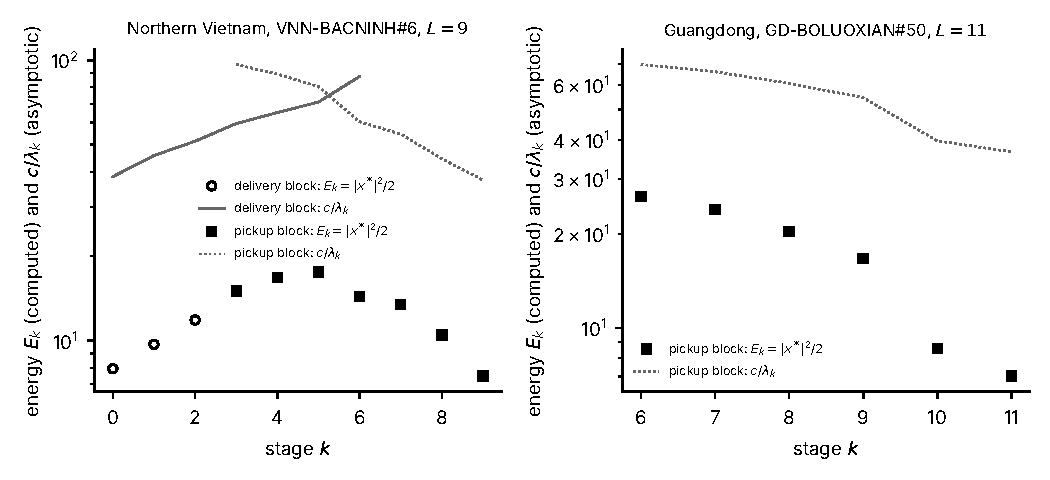
\includegraphics[width=0.85\textwidth]{figures/rarecert_mode_energies.pdf}
\caption{Computed dominating-point energies $E_k=\min\{|u|^2/2:L_k(u)\ge c\}$ of the stage
events (open circles: delivery block; filled squares: pickup block) against the stage
$k$, with the asymptotic value $c/\lambda_k$ (lines), at level $10^{-4}$. Left: a route
with balanced pickups and deliveries ($\varrho=0.93$), with two end modes of nearly
equal energy. Right: a route whose pickups are $2.7$ times its deliveries; no delivery
block reaches $c$ in the simulator, whose normal scores are clipped at $\Phi^{-1}(1-10^{-15})$.}
\label{fig:energies}
\end{figure}

\section{A single mean shift}
\label{sec:single}

Importance sampling with proposal $q$ estimates $p=\P(A)$ by
$\hat p_N=N^{-1}\sum_{j\le N}\one_A(U_j)\,\varphi(U_j)/q(U_j)$, $U_j\sim q$ i.i.d.; its second
moment per draw is $m_2=\int_A\varphi^2/q$. The estimator is \emph{logarithmically
efficient} if $\log m_2/(2\log p)\to1$ \citep{AsmussenGlynn2007}. For the mean shift
$q=\varphi(\cdot-\tau)$ the likelihood ratio is $w(u)=e^{-\ip u\tau+|\tau|^2/2}$. All our
proposals are mixtures $q=\sum_ma_m\varphi(\cdot-\tau_m)$, $a_m>0$, $\sum a_m=1$, and we
bound $m_2$ through
\[
J_m(u)=\tfrac12|u+\tau_m|^2-|\tau_m|^2,\qquad \Upsilon(u)=\max_m\big(J_m(u)+\log a_m\big).
\]

\begin{lemma}[Second moment of a mixture]\label{lem:m2}
$m_2\le(2\pi)^{-n/2}\int_Ae^{-\Upsilon(u)}du$. If $\Upsilon\ge\gamma_0>0$ on $A$, then for every
component $m$,
$m_2\le a_m^{-1}C_n\,(1+\gamma_0+|\tau_m|^2)^{n/2}e^{-\gamma_0}$ with $C_n$ depending on $n$
only.
\end{lemma}

\begin{proof}
$\varphi^2/q\le\min_m\varphi^2/(a_m\varphi(\cdot-\tau_m))$ and
$\varphi(u)^2/\varphi(u-\tau)=(2\pi)^{-n/2}e^{-J(u)}$, which gives the first bound. Fix $m$.
On $A$, $\Upsilon\ge\max(\gamma_0,J_m+\log a_m)\ge\max(\gamma_0,J_m)+\log a_m$, so
$m_2\le a_m^{-1}(2\pi)^{-n/2}e^{|\tau_m|^2}\int e^{-\max(\gamma_0+|\tau_m|^2,|v|^2/2)}dv$
after the substitution $v=u+\tau_m$. With $R^2=2(\gamma_0+|\tau_m|^2)$, the integral is
at most $V_nR^ne^{-R^2/2}+(2\pi)^{n/2}\P(\chi^2_n>R^2)$, and both terms are
$O((1+R^2)^{n/2}e^{-R^2/2})$.
\end{proof}

Write $\lambda_{\rm o}=\varrho\lambda^\star$ for the weaker end scale and let $e^\star$ be
the Perron direction of the dominant end block, $\mu^\star$ its second eigenvalue, and
$\tau^\star=\sqrt{2c/\lambda^\star}\,e^\star$ the asymptotic dominating point.

\begin{theorem}\label{thm:single}
\begin{enumerate}
\item[(a)] Let $\tau$ be any vector supported on the inputs of the dominant end's type
(the delivery inputs $W_d,E_{d,\cdot}$ when the dominant end is the delivery block; for
instance $\tau^\star$). Then
$\log m_2\ge|\tau|^2-c/\lambda_{\rm o}-O(\sqrt c)$. For $\tau=\tau^\star$,
\[
\log m_2-2\log p\ \ge\ \frac{c}{\lambda^\star}\Big(4-\frac1\varrho\Big)-O(\sqrt c),
\]
so the shift $\tau^\star$ is not logarithmically efficient if $\varrho>1/4$.
\item[(b)] For the defensive version $q=a_0\varphi+(1-a_0)\varphi(\cdot-\tau^\star)$ with a
fixed $a_0\in(0,1)$, $\log m_2\ge-c/\lambda_{\rm o}-O(\sqrt c)$, so it is not
logarithmically efficient if $\varrho>1/2$.
\item[(c)] If $\varrho\le1/4$ and $\mu^\star\le\lambda^\star/4$, the shift $\tau^\star$ is
logarithmically efficient; indeed $\log m_2\le-2c/\lambda^\star+O(\log c)$.
\end{enumerate}
\end{theorem}

\begin{proof}
Say the dominant end is the delivery block at stage $0$; the other case is symmetric. Let
$\mathcal{B}=\{P_L>c\}\subseteq A$, an event of the pickup inputs only, with
$\log\P(\mathcal{B})=-c/\lambda_{\rm o}+O(\sqrt c)$ by Theorem~\ref{thm:ld}.

(a) $w$ depends on the delivery inputs only, so by independence
\[
m_2\ge\E[w\one_{\mathcal{B}}]=\E[w]\,\P(\mathcal{B})=e^{|\tau|^2}\P(\mathcal{B}).
\]
With $|\tau^\star|^2=2c/\lambda^\star$
and $\log p=-c/\lambda^\star+O(\sqrt c)$ the display follows, and then
$\limsup\log m_2/(2\log p)\le1-(4-1/\varrho)/2<1$ when $\varrho>1/4$.

(b) Here $w=1/(a_0+(1-a_0)e^{\ip u{\tau^\star}-|\tau^\star|^2/2})\ge1$ on
$\{\ip u{\tau^\star}\le|\tau^\star|^2/2\}$, an event of the delivery inputs of probability at
least $1/2$; by independence $m_2\ge\frac12\P(\mathcal{B})$. Efficiency would need
$\log m_2\le-2c/\lambda^\star+o(c)$, which fails when $1/\lambda_{\rm o}<2/\lambda^\star$.

(c) Since $F\le D_0+P_L$, Lemma~\ref{lem:quantile} gives
$A\subseteq\{h_{S^d_0}(u)+h_{S^p_L}(u)\ge c-C\log(2+|u|)-C\}$. Apply Lemma~\ref{lem:block}
to the dominant block with $a=\ip u{e^\star}$, and bound the other block, of matrix
$M_{\rm o}$ and projection $\Pi_{\rm o}$, by
$h\le\frac12u^\top M_{\rm o}u\le\frac12\lambda_{\rm o}|\Pi_{\rm o}u|^2$; the two blocks read
disjoint coordinates, so $|u^\perp|^2+|\Pi_{\rm o}u|^2\le|u|^2-a^2$. With $g^2=|u|^2-a^2$ and
$\nu'=\max(\mu^\star,\lambda_{\rm o})/\lambda^\star\le1/4$,
\[
2(h_{S^d_0}+h_{S^p_L})(u)\le\lambda^\star(a_+^2+\nu'g^2).
\]
The single component has $J(u)=\frac12|u+\tau^\star|^2-|\tau^\star|^2$. Let $R=4|\tau^\star|$. If
$|u|>R$ then $J(u)\ge\frac12(3|\tau^\star|)^2-|\tau^\star|^2>2c/\lambda^\star$. If $|u|\le R$,
then $u\in A$ implies $a_+^2+\nu'g^2\ge2c'/\lambda^\star$ with $c'=c-O(\log c)$. Scale
$y=u\sqrt{\lambda^\star/c'}$, so that $a_{y,+}^2+\nu'g_y^2\ge2$, $|y|=O(1)$ and
$J(u)=\frac{c'}{2\lambda^\star}\big(|y+\sigma\sqrt2e^\star|^2-4\sigma^2\big)$ with
$\sigma^2=c/c'=1+O(\log c/c)$. We claim $|y+\sqrt2e^\star|^2-4\ge4$ under the
constraint. If $a_y\ge0$, then $g_y^2\ge4(2-a_y^2)_+$ and
$|y+\sqrt2e^\star|^2-4=a_y^2+2\sqrt2a_y-2+g_y^2\ge6-3a_y^2+2\sqrt2a_y\ge4$ for
$a_y\le\sqrt2$ (a concave function equal to $6$ and $4$ at the endpoints), and
$\ge(2\sqrt2)^2-4=4$ for $a_y>\sqrt2$. If $a_y<0$, then $g_y^2\ge8$ and the left side is
at least $g_y^2-4\ge4$. Replacing $\sqrt2$ by $\sigma\sqrt2$ changes the left side by
$O(\sigma-1)$ on $|y|=O(1)$, so $J\ge2c/\lambda^\star-O(\log c)$ on $A$, and
Lemma~\ref{lem:m2} gives the bound. Since $m_2\ge p^2$, efficiency follows from
Theorem~\ref{thm:ld}.
\end{proof}

The threshold $1/4$ in (a) and (c) is sharp in $\varrho$; the extra condition on
$\mu^\star$ in (c) is a spectral gap of the dominant block, which by
Lemma~\ref{lem:spectral}(b) holds when
$\rho\sum\theta_i+(1-\rho)\min\theta\ge4(1-\rho)\max\theta$. The proof of (a) also shows
where the second moment comes from: draws with typical delivery inputs and pickup inputs in
$\mathcal{B}$, which carry weight $e^{-\ip u\tau+|\tau|^2/2}$ but are proposed no more often than
under crude Monte Carlo. That has a consequence for what a user sees.

\begin{proposition}[Silent underestimation]\label{prop:silent}
Let $q$ be any proposal under which the pickup inputs keep their standard normal law,
independent of the delivery inputs (for instance a shift supported on the delivery
inputs, with or without a defensive component, or the two-step scheme of
\citet{GlassermanLi2005} with its factor and inner shifts taken from the delivery end
mode, whose dominating point has no pickup coordinates), and let
$\mathcal{B}=\{P_L>c\}$, $p_{\mathcal{B}}=\P(\mathcal{B})$. Then $q(\mathcal{B})=p_{\mathcal{B}}$, and for the estimator $\hat p_N$,
\[
\P_q(\text{no draw in }\mathcal{B})=(1-p_{\mathcal{B}})^N\ge1-Np_{\mathcal{B}},\qquad
\E_q\big[\hat p_N\,\big|\,\text{no draw in }\mathcal{B}\big]=\frac{p-p_{\mathcal{B}}}{1-p_{\mathcal{B}}}.
\]
So on an event of probability at least $1-Np_{\mathcal{B}}$ the estimator has conditional mean
$p(1-s)(1+O(p))$, where $s=p_{\mathcal{B}}/p$ is the share of the weaker end event, and the
sample variance it reports is computed from draws that all avoid $\mathcal{B}$, so it estimates the
variance under $q(\cdot\mid \mathcal{B}^c)$, not $m_2$. The symmetric statement holds with
deliveries and pickups exchanged.
\end{proposition}

\begin{proof}
$q(\mathcal{B})=p_{\mathcal{B}}$ because $\mathcal{B}$ is an event of the pickup inputs. Given that no draw falls in
$\mathcal{B}$ the draws are i.i.d.\ from $q(\cdot\mid \mathcal{B}^c)$, and
$\E_q[\one_Aw\mid \mathcal{B}^c]=\int_{A\setminus \mathcal{B}}\varphi\big/(1-p_{\mathcal{B}})=(p-p_{\mathcal{B}})/(1-p_{\mathcal{B}})$, because
$\mathcal{B}\subseteq A$. Finally $(p-p_{\mathcal{B}})/(1-p_{\mathcal{B}})=p(1-s)(1+O(p))$.
\end{proof}

The proposition explains three facts reported in Section~\ref{sec:numerics}: the single
shift underestimates by about the share $s$ of the weaker end mode; its reported standard
error does not reveal this, because the variance it estimates is that of a sample that
avoids $\mathcal{B}$; and Glasserman--Li two-step sampling, which shifts the dominant factor only,
has the same bias. Unbiasedness is restored only through rare draws in $\mathcal{B}$, each
carrying a weight of order $e^{-\ip u\tau+|\tau|^2/2}$. By Corollary~\ref{cor:ends},
$s=\exp\{-c(1/\lambda_{\rm o}-1/\lambda^\star)+O(\sqrt c)\}$, so the bias is negligible
for small $\varrho$ and of order one for $\varrho$ near $1$, while the threshold of
Theorem~\ref{thm:single}(a) is $1/4$: variance inflation and visible bias are different
regimes.

\section{Stage mixtures}
\label{sec:mixture}

A mixture places components at the dominating points of several stage blocks. For a
stage $k$ and a block $b$ of it, the asymptotic dominating point of $\{h_{S^b_k}\ge c\}$
is $\tau_{k,b}=\sqrt{2c/\lambda^b_k}\,e_{S^b_k}$, and we consider
\[
q=a_0\varphi+\sum_{m\in\mathcal M}a_m\varphi(\cdot-\tau_m),\qquad
a_0\in(0,1)\text{ fixed},\quad a_m=e^{-c\delta_m+o(c)},\ \delta_m\ge0,
\]
for a set $\mathcal M$ of (stage, block) pairs. Constant weights have $\delta_m=0$; weights
proportional to the asymptotic mode masses, $a_m\propto e^{-c/\lambda_m}$, have
$\delta_m=1/\lambda_m-1/\lambda^\star$.

\begin{definition}[Covering constant]\label{def:psi}
For $\varrho\in[0,1]$, $\nu\in[0,1]$ and penalties $\pi_H,\pi_W\in[0,\infty]$ let
\begin{align*}
F_0(a,b,g)&=a^2+b^2+g^2,\\
F_H(a,b,g)&=(a+\sqrt2)^2+b^2+g^2-4-\pi_H,\\
F_W(a,b,g)&=a^2+\big(b+\sqrt{2/\varrho}\big)^2+g^2-4/\varrho-\pi_W,
\end{align*}
and
$\Psi(\varrho,\nu;\pi_H,\pi_W)=\inf\{\max(F_0,F_H,F_W):\ a,b\in\R,\ g\ge0,\
a_+^2+\varrho b_+^2+\nu g^2\ge2\}$,
with $F_W$ omitted when $\varrho=0$ or $\pi_W=\infty$ and $F_H$ omitted when
$\pi_H=\infty$. We write $\psi(\varrho,\nu)=\Psi(\varrho,\nu;0,0)$ (both blocks, constant
weights) and $\psi_H(\varrho,\nu)=\Psi(\varrho,\nu;0,\infty)$ (dominant block only).
\end{definition}

Every function in the maximum increases in $g$, so for $\nu>0$ the infimum over $g$ is
attained at $g^2=(2-a_+^2-\varrho b_+^2)_+/\nu$ (for $\nu=0$ the constraint forces
$a_+^2+\varrho b_+^2\ge2$ and $g=0$), and $\Psi$ is the minimum of an explicit function of
two variables; it is evaluated numerically in seconds.

\begin{lemma}\label{lem:psi}
Let $\varrho,\nu\in[0,1]$.
\begin{enumerate}
\item[(a)] $2\le\Psi\le4$ whenever $\pi_H=0$; with no components ($\pi_H=\pi_W=\infty$)
$\Psi\ge2$.
\item[(b)] If $\varrho\le1/3$ and $\nu\le1/3$, then $\psi_H(\varrho,\nu)=\psi(\varrho,\nu)=4$.
\item[(c)] If $\nu\le1/2$, then $\psi(\varrho,\nu)\ge2\sqrt2$, with equality at $\varrho=1$.
\item[(d)] For a stage with one block only ($\varrho=0$) and $\nu\in(0,1]$,
$\psi_H(0,\nu)=\min\big(4,\tfrac12+\tfrac3{2\nu}\big)$; it equals $4$ iff $\nu\le3/7$.
\end{enumerate}
\end{lemma}

\begin{proof}
(a) $F_0\ge a_+^2+\varrho b_+^2+\nu g^2\ge2$. At $(a,b,g)=(\sqrt2,0,0)$, $F_0=2$, $F_H=4$ and
$F_W=2-2/\varrho\le0$.

In (b) and (c) write $X=a_+^2$, $Y=\varrho b_+^2$, $W=\nu g^2$, so that $X+Y+W\ge2$, and
note $b^2\ge Y/\varrho$, $g^2=W/\nu$.

(b) If $a>0$: $F_H\ge X+2\sqrt{2X}-2+3(Y+W)\ge X+2\sqrt{2X}-2+3(2-X)_+$, which is at
least $4$: for $X\le2$ it is the concave function $4-2X+2\sqrt{2X}$, equal to $4$ at both
ends, and for $X>2$ it exceeds $2+4-2$. If $a\le0$: $Y+W\ge2$ and
$F_0\ge b^2+g^2\ge3(Y+W)\ge6$. With (a), $\psi_H=4$; adding $F_W$ cannot lower the
maximum, and $\psi\le4$ by (a).

(c) Here $g^2\ge2W$, and let $y_0=(2-\sqrt2)^2$, the root of $Y+2\sqrt{2Y}=2$; the
monotonicity in $X,Y,W$ allows us to assume $X+Y+W=2$.
\emph{Case $a,b>0$.} $F_0\ge X+Y+2W$, $F_H\ge X+2\sqrt{2X}-2+Y+2W$ and
$F_W=X+g^2+(Y+2\sqrt{2Y}-2)/\varrho$. If $Y\ge y_0$, the last bracket is nonnegative and
$F_W\ge X+2\sqrt{2Y}-2+Y+2W$; with $S=X+Y$ and $\max(\sqrt X,\sqrt Y)\ge\sqrt{S/2}$,
$\max(F_0,F_H,F_W)\ge\max(4-S,\,2-S+2\sqrt S)$, which is at least $3$ for $S\le1$ and at
least $2\sqrt2$ on $[1,2]$ (concavity; the value at $S=2$ is $2\sqrt2$). If $Y<y_0$:
either $W\ge2\sqrt2-2$, and $F_0\ge2+W\ge2\sqrt2$, or $X\ge2-y_0-W$ and
$F_H\ge W+2\sqrt{2X}\ge W+2\sqrt{2(2-y_0-W)}$, a concave function of
$W\in[0,2\sqrt2-2]$ whose end values are $3.64$ and $3.40$.
\emph{Case $a\le0<b$.} Then $Y+W=2$ and, dropping $a^2$, $F_W\ge(Y+2\sqrt{2Y}-2)/\varrho+2W$.
If $Y\ge y_0$, $F_W\ge2-Y+2\sqrt{2Y}\ge3.31$ on $[y_0,2]$; if $Y<y_0$,
$F_0\ge Y+2W=4-Y>3.6$. \emph{Case $b\le0<a$} is the same with $F_H$.
\emph{Case $a,b\le0$.} $F_0\ge g^2\ge2/\nu\ge4$.
Equality at $\varrho=1$: at $a=b=1$, $g=0$ we get $F_0=2$ and $F_H=F_W=2\sqrt2$.

(d) With $\varrho=0$ the constraint is $a_+^2+\nu g^2\ge2$ (the coordinate $b$ is part of
$g$). If $a\le0$, $F_0\ge g^2\ge2/\nu\ge\frac12+\frac3{2\nu}$. If $a>0$, put $X=a^2$; both
functions increase in $g$, so take $g^2=(2-X)_+/\nu$. Then $F_H\ge F_0$ iff $X\ge1/2$. On
$[0,1/2]$ the maximum is $F_0=X+(2-X)/\nu$, decreasing in $X$, with value
$\frac12+\frac3{2\nu}$ at $X=1/2$; on $[1/2,2]$ it is $F_H=X(1-1/\nu)+2\sqrt{2X}-2+2/\nu$,
concave, with end values $\frac12+\frac3{2\nu}$ and $4$; for $X>2$, $F_H>4$. The infimum
is the smaller end value, attained.
\end{proof}

\begin{theorem}\label{thm:mixture}
For each stage $k$ let $\pi_H=2\lambda_k\delta_m$ if the dominant block $m=(k,H)$ of the
stage belongs to $\mathcal M$ and $\pi_H=\infty$ otherwise, $\pi_W$ likewise for the weak
block, and $\Psi_k=\Psi(\varrho_k,\nu_k;\pi_H,\pi_W)$. If
\begin{equation}\label{eq:cover}
\Psi_k\ \ge\ 4\,r_k=4\lambda_k/\lambda^\star\qquad\text{for every stage }k=0,\dots,L,
\end{equation}
then $\log m_2\le-2c/\lambda^\star+o(c)$, and the mixture estimator is logarithmically
efficient. With constant weights the error term is $O(\log c)$.
\end{theorem}

\begin{proof}
By Lemma~\ref{lem:m2} applied with the defensive component $m=0$ (whose weight $a_0$ is
fixed) it suffices to show
$\Upsilon(u)\ge2c/\lambda^\star-o(c)$ on $A$. Since $\Upsilon\ge J_0+\log a_0=|u|^2/2+\log a_0$,
this holds for $|u|>R:=3\sqrt{c/\lambda^\star}$, and we take $u\in A$ with $|u|\le R$.
Then $u\in\{L_k>c\}$ for some $k$, and by \eqref{eq:sandwich-k} and
\eqref{eq:stage-form}, $a_+^2+\varrho_kb_+^2+\nu_kg^2\ge2c'/\lambda_k$ with
$c'=c-O(\log c)$, in the coordinates of stage $k$. Put $y=u\sqrt{\lambda_k/c'}$ and
$\sigma^2=c/c'$. In these coordinates the components of the stage are
$\tau_{k,H}=\sqrt{c'/\lambda_k}\,\sigma\sqrt2\,e_H$ and
$\tau_{k,W}=\sqrt{c'/\lambda_k}\,\sigma\sqrt{2/\varrho_k}\,e_W$, and
\[
J_0(u)=\frac{c'}{2\lambda_k}F_0(y),\qquad
J_{k,H}(u)+\log a_{k,H}=\frac{c'}{2\lambda_k}F^\sigma_H(y)+o(c),
\]
where $F^\sigma_H$ is $F_H$ with $\sqrt2$ replaced by $\sigma\sqrt2$, $4$ by $4\sigma^2$ and
$\pi_H=2\lambda_k\delta_{k,H}$ by $2\lambda_k\delta_{k,H}c/c'$; likewise for $W$. Since
$|y|=O(1)$ and $\sigma\to1$, $F^\sigma\ge F-o(1)$ uniformly, so
$\Upsilon(u)\ge\frac{c'}{2\lambda_k}(\Psi_k-o(1))\ge\frac{2c}{\lambda^\star}-o(c)$ by
\eqref{eq:cover}. With $\delta_m=0$ the $o(\cdot)$ terms are $O(\log c)$, as in the proof
of Theorem~\ref{thm:single}(c).
\end{proof}

\begin{corollary}\label{cor:closed}
With constant weights, \eqref{eq:cover} holds at stage $k$ if (i) $r_k\le1/2$, with no
component for the stage; or (ii) $\varrho_k\le1/3$, $\nu_k\le1/3$ and the dominant block
of the stage is in $\mathcal M$; or (iii) $r_k\le1/\sqrt2$, $\nu_k\le1/2$ and both blocks
of the stage are in $\mathcal M$.
\end{corollary}

\begin{proof}
Lemma~\ref{lem:psi}(a), (b) and (c).
\end{proof}

\begin{remark}
(1) The end stages need components. Stage $0$ has an empty pickup block ($\varrho_0=0$,
$r_0=\lambda^d_0/\lambda^\star$), so by Lemma~\ref{lem:psi}(d) the delivery end
component covers it iff $\frac12+\frac3{2\nu_0}\ge4r_0$; at the dominant end ($r_0=1$)
this is the gap condition $\nu_0\le3/7$. The same holds at stage $L$. For mass
weights, at an end stage with no weak block and $\nu_k\le1/3$, the proof of
Lemma~\ref{lem:psi}(b) gives $F_H-\pi_H\ge4-2(1-r_k)=2+2r_k\ge4r_k$ where $F_H$ covers,
and $F_0\ge6$ elsewhere; so the penalties do not hurt at the ends.
(2) Interior stages close to an end have $\varrho_k$ small and are covered by (ii); the
crossing stage, where the two blocks are comparable, has $r_k$ near $1/2$ on routes with
many stops, because the scales are close to $\rho\sum\theta$ and the stage splits the route
(Lemma~\ref{lem:spectral}(b)). For ties with $r_k>1/\sqrt2$ the covering inequality fails with two
components and constant weights ($\psi=2\sqrt2<4r_k$ by Lemma~\ref{lem:psi}(c)), so
Theorem~\ref{thm:mixture} gives no guarantee; a continuum of components along the arc
between the two block directions is the natural remedy, in the spirit of
\citet{DupuisWang2007}. We do not pursue this, because it does not occur on our routes at
$\rho\ge0.6$ (Table~\ref{tab:conditions}).
(3) The theorem is stated for the asymptotic dominating points. Its proof uses the shifts
only through $\tau_m/\sqrt c$, so it remains true for any shifts with
$\tau_m(c)=\tau_{m}+o(\sqrt c)$. We do not prove that the computed minimisers used in
practice satisfy this.
\end{remark}

\begin{corollary}[Several routes]\label{cor:plan}
Let routes $j=1,\dots,J$ share the factors $W_d,W_p$ and have their own idiosyncratic
inputs, with capacities $c_j=\alpha_jc$ for fixed $\alpha_j>0$. Then
$\log\P(\bigcup_j\{F_j>c_j\})=-c\min_j\alpha_j/\lambda^\star_j+O(\sqrt c)$, and the
mixture over the stage components of all routes is logarithmically efficient if
\eqref{eq:cover} holds for every route and stage with $\lambda^\star$ replaced by
$\max_j\lambda^\star_j/\alpha_j$ and $\lambda_k$ by $\lambda_{j,k}/\alpha_j$.
\end{corollary}

\begin{proof}
Each stage event involves one route, and the input coordinates of its two blocks are
still disjoint from each other; the proofs of Theorems~\ref{thm:ld} and~\ref{thm:mixture}
apply to the finite union over (route, stage) pairs, after rescaling the capacities.
\end{proof}

\section{Numerical illustration}
\label{sec:numerics}

\subsection{Setting}
We use the routes of plans for two regions, built by an adaptive large-neighbourhood
search on road-network instances: 26 depot areas in Northern Vietnam (375 routes, 2\,612
customers, capacity $15$\,t) and 122 in Guangdong (5\,867 routes, 37\,487 customers,
$30$\,t). The mean demands come from regional parcel statistics; in Vietnam the pickup
rate equals the delivery rate (no regional figure is published), in Guangdong pickups
are on average $2.7$ times the deliveries. Routes have $6$--$7$ stops in median and up to
$40$. The demand model is that of Section~\ref{sec:model} with coefficient of variation
$0.3$ and $\rho=0.6$, and we vary $\rho$ and the coefficient of variation in
Section~\ref{sec:checks}. Normal scores are clipped at $\Phi^{-1}(1-10^{-15})$ in the
simulator; this changes each input's law on a set of probability $10^{-15}$ and every
probability below by less than $10^{-13}$. The two regions differ in $\varrho$:
median $0.93$ in Vietnam (balanced routes) and $0.36$ in Guangdong.

\emph{Estimators.} SMIS is the stage mixture of Section~\ref{sec:mixture} with three
practical choices: the shifts are computed minimisers of $|u|^2/2$ over $\{L_k\ge c\}$
(SLSQP, started on the block's Perron ray, with the exact quantile transform); a mode is
kept if its computed energy $E_m$ is within $\log(1/\eta)$ of the smallest,
$\eta=10^{-3}$; and the weights are $a_m\propto e^{-(E_m-E_{\min})}$, the finite-level
analogue of mass weights, with a defensive weight $a_0=0.05$. There is no pilot run. We
compare it with the single shift at the dominant end tuned by the multilevel
cross-entropy (CE) method \citep{deBoerEtAl2005}, a CE mixture with one CE shift per
stage, Glasserman--Li two-step sampling \citep{GlassermanLi2005} with the factor shift at
the dominant point and an inner exponential shift, conditional Monte Carlo over the two
factors with an inner dynamic program, and subset simulation \citep{AuBeck2001}. The
reference is a quadrature program: given the two factors the demands are independent,
so $\P(F>c\mid W_d,W_p)$ is a one-dimensional dynamic program on a discretised load
($256$ and $512$ levels with Richardson extrapolation), integrated by a product
trapezoid rule on $[-6,9]^2$; its error estimate is below $1\%$ of $p$ at the grids used.
Capacities are set so that $p\approx\gamma\in\{10^{-3},10^{-4},10^{-5},10^{-6}\}$.

\subsection{The conditions on real routes}
Table~\ref{tab:conditions} evaluates the conditions of Theorems~\ref{thm:single}
and~\ref{thm:mixture} on all 5\,920 routes with at least two stops. Every route has
$\varrho>1/4$, so the single shift is never efficient: the threshold of
Theorem~\ref{thm:single} is not informative about which routes fail in practice; the
share $s$ of Proposition~\ref{prop:silent} is. With constant weights the covering condition~\eqref{eq:cover}
holds for every route at $\rho=0.6$ and $0.8$, with a smallest margin $\Psi_k-4r_k$ of
$0.23$ at $\rho=0.6$ among the stages that need the exact constant; the closed-form
conditions of Corollary~\ref{cor:closed} miss three quarters of the Vietnamese routes,
whose crossing stages have $r_k\in(0.71,0.90)$ and $\varrho_k\in(0.33,0.8)$. At $\rho=0.3$
the blocks have smaller spectral gaps and the condition holds for $86\%$ of the routes.
With mass weights, the finite-level analogue of which SMIS uses, it holds for every
Guangdong route at $\rho\ge0.6$ but for only $28\%$ of the Vietnamese routes at
$\rho=0.6$: on balanced routes the crossing stages carry a weak-block penalty that the
covering constant cannot absorb. Section~\ref{sec:checks} shows that SMIS is accurate
on these routes too, so the condition is sufficient, not necessary; for a guarantee on
balanced routes, constant weights on the crossing-stage components are the safe
choice.

\begin{table}[t]
\centering\small
\caption{Conditions of the theorems on all routes with at least two stops: median
end-mode ratio $\varrho$, share of routes with $\varrho>1/4$ (single shift not
efficient, Theorem~\ref{thm:single}), and share satisfying the covering
condition~\eqref{eq:cover} with components for both blocks of every stage with
$r_k>1/2$: by the closed-form cases of Corollary~\ref{cor:closed}, with the exact
constant $\psi$ and constant weights, and with mass weights
$\delta_m=1/\lambda_m-1/\lambda^\star$. The conditions do not depend on the coefficient
of variation.}
\label{tab:conditions}
\begin{tabular}{llrrrrrr}
\toprule
$\rho$ & region & routes & $\varrho$ & $\varrho>1/4$ & Cor.~\ref{cor:closed} & $\psi$, constant & $\Psi$, mass \\
\midrule
0.3 & Vietnam & 347 & 0.92 & 100.0\% & 0.0\% & 91.6\% & 0.3\% \\
0.3 & Guangdong & 5573 & 0.36 & 100.0\% & 3.3\% & 85.3\% & 84.0\% \\
0.6 & Vietnam & 347 & 0.93 & 100.0\% & 23.9\% & 100.0\% & 27.7\% \\
0.6 & Guangdong & 5573 & 0.36 & 100.0\% & 99.9\% & 100.0\% & 100.0\% \\
0.8 & Vietnam & 347 & 0.93 & 100.0\% & 52.4\% & 100.0\% & 63.7\% \\
0.8 & Guangdong & 5573 & 0.37 & 100.0\% & 100.0\% & 100.0\% & 100.0\% \\
\bottomrule
\end{tabular}
\end{table}


\subsection{The single shift and the missed end mode}
On 120 routes (80 from Guangdong, 40 from Vietnam, sampled with a fixed seed and
stratified by number of stops; $4$ to $15$ stops) and four levels, every estimator uses
$10^6$ draws. Table~\ref{tab:routes} reports the relative error against the quadrature
reference where it is available (routes with at most eight stops at $10^{-3}$ and
$10^{-4}$) and against the CE mixture otherwise. On routes with $\varrho\le0.5$ the single
shift is as accurate as the mixtures; on the balanced routes ($\varrho>0.75$) its median
error is $3$--$6\%$, with $90\%$ quantiles up to $40\%$, and it underestimates in
$93$--$95\%$ of the rows at $\gamma\le10^{-4}$. Its sample relative variance reveals the
problem at $10^{-3}$ and $10^{-4}$ (512 and 87, against 4--5 for SMIS) but not at
$10^{-5}$ and $10^{-6}$ (5.2 and 5.5), as Proposition~\ref{prop:silent} predicts once
$Np_B$ is small. The relative variance of SMIS grows from $3.8$ to $5.9$ over three
decades of $\gamma$, consistent with logarithmic efficiency.

\begin{table}[t]
\centering\small
\caption{120 routes, $10^6$ draws: absolute relative error (median / $90\%$ quantile)
and sample relative variance (median) by band of $\varrho$. The reference is the
quadrature program for 178 of the 480 rows and the CE mixture for the others, so the CE
mixture has no entry at $\gamma\le10^{-5}$. One route in $(0.5,0.75]$ is omitted.}
\label{tab:routes}
\begin{tabular}{llrrrrrr}
\toprule
$\gamma$ & $\varrho$ & $n$ & SMIS & CE mixture & single shift & RV SMIS & RV single \\
\midrule
$10^{-3}$ & $\le0.5$ & 79 & 0.14 / 0.38\% & 0.09 / 0.33\% & 0.18 / 0.45\% & 3.77 & 3.51 \\
          & $>0.75$  & 40 & 0.22 / 0.44\% & 0.05 / 0.32\% & 2.86 / 7.57\% & 4.05 & 512 \\
$10^{-4}$ & $\le0.5$ & 79 & 0.17 / 0.46\% & 0.13 / 0.40\% & 0.18 / 0.48\% & 4.51 & 4.23 \\
          & $>0.75$  & 40 & 0.20 / 0.42\% & 0.07 / 0.36\% & 5.10 / 21.7\% & 4.71 & 87 \\
$10^{-5}$ & $\le0.5$ & 79 & 0.20 / 0.48\% & ref. & 0.16 / 0.51\% & 5.18 & 4.88 \\
          & $>0.75$  & 40 & 0.26 / 0.58\% & ref. & 6.00 / 26.7\% & 5.31 & 5.22 \\
$10^{-6}$ & $\le0.5$ & 79 & 0.26 / 0.56\% & ref. & 0.23 / 0.56\% & 5.79 & 5.46 \\
          & $>0.75$  & 40 & 0.22 / 0.52\% & ref. & 6.05 / 39.9\% & 5.88 & 5.50 \\
\bottomrule
\end{tabular}
\end{table}

\emph{The share predicts the error.} Proposition~\ref{prop:silent} says that, on the
typical event, the single shift and the Glasserman--Li estimator have mean
$p(1-s)$, with $s=\P(\text{weaker end event})/p$. We estimated both end probabilities for the 30 routes of
Table~\ref{tab:rivals} at $10^{-4}$ and $10^{-6}$ on the single blocks (the route with its
pickups, respectively deliveries, set to zero), where there is one mode and SMIS has a
relative standard error of about $0.2\%$ with $10^6$ draws (Table~\ref{tab:bias}). In the 47 route--level rows where an estimator expects fewer than one draw in the weaker mode ($Np_{\mathcal B}<1$), its underestimate follows $s$: the Spearman correlation is $0.92$ and the median ratio of underestimate to $s$ is $1.00$. The single shift at $10^{-4}$ expects about $14$ such draws in median; it then reaches the weaker mode, and the deficit shows partly as error and partly as variance (relative variance $212$ in Table~\ref{tab:rivals}). On the routes with $\varrho\le0.75$, $s<10^{-15}$ and both estimators are unbiased within their sampling error.

A cheaper proxy, available without quadrature, is
$\hat m=\exp\{-(E_{\rm o}-E_{\min})\}$ with the computed energies of the two end modes; over
all 480 route--level rows the absolute error of the single shift is at the noise level
when $\hat m<10^{-6}$ (all Guangdong) and about $0.8\,\hat m$ when $\hat m\ge10^{-2}$
(Figure~\ref{fig:mhat}). The retention rule of SMIS keeps exactly the modes with
$\hat m\ge\eta$, so by the same proposition the modes it drops carry a share of order
$\eta$ at most.

\begin{table}[t]
\centering\small
\caption{Silent underestimation on the 15 balanced routes ($\varrho>0.75$) of
Table~\ref{tab:rivals}. $p_{\mathcal B}$ is the probability of the weaker end event,
estimated on the single block, and $s=p_{\mathcal B}/p$ its share, with $p$ the quadrature
reference; $Np_{\mathcal B}$ is the expected number of draws that reach that mode.
Underestimate: $-(\hat p-p)/p$. Ratio: underestimate$/s$ on the rows with $s>0.01$. All
medians over routes; last column: routes with $Np_{\mathcal B}<1$.}
\label{tab:bias}
\begin{tabular}{llrrrrrr}
\toprule
estimator & $\gamma$ & $N$ & $Np_{\mathcal B}$ & $s$ & underestimate & ratio & $Np_{\mathcal B}<1$ \\
\midrule
single CE shift & $10^{-4}$ & $10^6$ & 14 & 0.139 & 6.2\% & 0.90 & 2 \\
single CE shift & $10^{-6}$ & $10^6$ & 0.085 & 0.086 & 9.7\% & 1.02 & 15 \\
Glasserman--Li & $10^{-4}$ & $2\times10^4$ & 0.28 & 0.139 & 15.5\% & 1.05 & 15 \\
Glasserman--Li & $10^{-6}$ & $2\times10^4$ & 0.0017 & 0.086 & 7.4\% & 0.97 & 15 \\
\bottomrule
\end{tabular}
\end{table}


\begin{figure}[t]
\centering
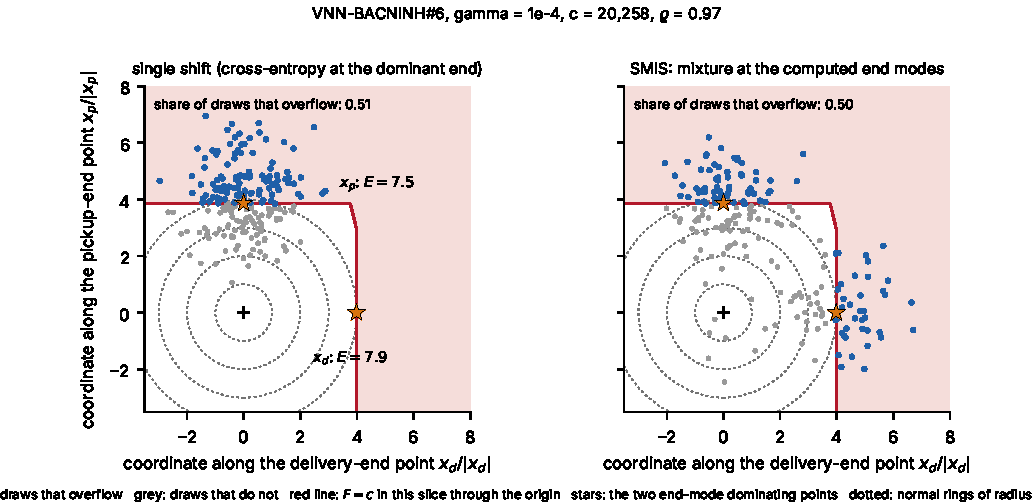
\includegraphics[width=0.48\textwidth]{figures/rarecert_geometry.pdf}\hfill
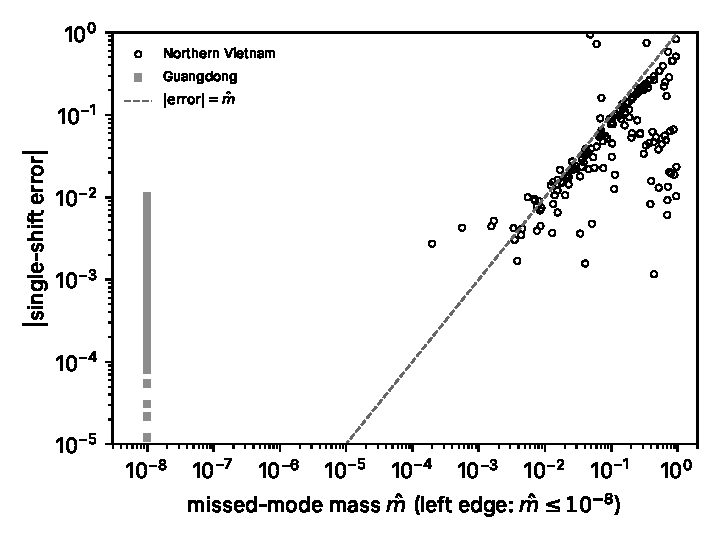
\includegraphics[width=0.48\textwidth]{figures/rarecert_mhat_all.pdf}
\caption{Left: the two end modes of a balanced route at $10^{-4}$ in the plane of the
two computed dominating points (shaded: the overflow set in this slice; stars: the two
dominating points); a single shift at one star reaches the other mode only as often as
crude sampling does. Right: absolute error of the single CE shift against the computed
weaker-mode mass $\hat m$, all 480 route--level rows (circles: Vietnam; squares:
Guangdong, all with $\hat m\le10^{-8}$, drawn at the left edge), with the line
$|\text{error}|=\hat m$.}
\label{fig:mhat}
\end{figure}

\subsection{Rivals, longer routes, coverage}
\label{sec:checks}
Table~\ref{tab:rivals} compares all methods on 30 of the routes (15 with
$\varrho>0.75$) against the quadrature reference. SMIS agrees with the reference within
$0.58\%$ on every route at both levels. Both factor-based rivals inherit the missed
mode: on the balanced routes the Glasserman--Li estimator is off by $15\%$ ($10^{-4}$) and
$6.6\%$ ($10^{-6}$) in median even with $10^6$ draws, where its sampling error is about
$0.5\%$, and the relative variance of conditional Monte Carlo jumps from about $1$ to
$57$--$153$. Subset simulation needs no mode information but has a relative variance of
$700$--$4\,400$ per draw. The quadrature program itself needs about $38$\,s per route and
level at the grid that keeps its error below $1\%$, against $2.5$\,s for SMIS at $1\%$
precision (one core); it does not extend to models in which the overflow event couples
loads with other random quantities, while the mixture does.

\begin{table}[t]
\centering\small
\caption{30 routes against the quadrature reference: absolute relative error (median /
maximum), relative variance per unit of work (median), and the one-core time for $1\%$
precision at $95\%$ confidence including build and pilot (median, s; measured on a shared
machine). Glasserman--Li: factor shift at the dominant point, inner exponential shift,
$2\times10^4$ draws.}
\label{tab:rivals}
\begin{tabular}{lrrrrrr}
\toprule
 & \multicolumn{3}{c}{$\gamma=10^{-4}$} & \multicolumn{3}{c}{$\gamma=10^{-6}$} \\
\cmidrule(lr){2-4}\cmidrule(lr){5-7}
method & error & RV & time & error & RV & time \\
\midrule
SMIS & 0.11 / 0.51\% & 4.6 & 2.6 & 0.16 / 0.58\% & 5.8 & 3.3 \\
CE mixture & 0.16 / 0.38\% & 4.6 & 4.6 & 0.29 / 0.85\% & 5.9 & 6.4 \\
single CE shift & 0.41 / 23.5\% & 4.3 & 2.5 & 0.36 / 94.7\% & 5.5 & 2.5 \\
Glasserman--Li & 3.1 / 47.1\% & 11 & 5.4 & 2.9 / 47.6\% & 13 & 6.6 \\
conditional Monte Carlo & 2.6 / 93.7\% & 6.5 & 9\,310 & 3.1 / 63.0\% & 1.4 & 2\,190 \\
subset simulation & 8.1 / 38.1\% & 716 & 431 & 21.6 / 108\% & 4\,430 & 1\,800 \\
\midrule
\multicolumn{7}{l}{routes with $\varrho>0.75$ only (15): median error} \\
SMIS & 0.15\% & 4.7 & & 0.15\% & 5.9 & \\
single CE shift & 6.2\% & 212 & & 9.7\% & 5.5 & \\
Glasserman--Li & 15.5\% & 12 & & 7.4\% & 13 & \\
\bottomrule
\end{tabular}
\end{table}

\emph{Two end modes suffice.} Keeping only the two end components of SMIS (same weights,
same defensive component) gives median errors of $0.08$--$0.19\%$ and relative variances
of $4.5$--$5.9$ on the same 30 routes, as accurate as the full mixture: at the levels of
interest the interior stages add nothing measurable, in line with
Corollary~\ref{cor:ends}.

\emph{Longer routes.} On eight routes with $15$ to $33$ stops, against crude Monte Carlo
with $5\times10^7$ draws at $10^{-3}$ and $10^8$ at $10^{-4}$ (relative standard errors
$0.45\%$ and $1.0\%$), SMIS deviates by at most $0.93\%$ and $1.5\%$, within two standard
errors of the reference. The single shift is accurate on the seven Guangdong routes
($\varrho\le0.41$) and fails on the balanced one ($\varrho=0.96$).

\emph{Model variations.} On 30 Guangdong routes at $10^{-4}$, SMIS stays within its
sampling error (median $0.27$--$0.43\%$ against a relative standard error of $0.47\%$)
for $\rho\in\{0.3,0.8\}$, coefficient of variation $0.2$ and $0.5$, pickups scaled by
$0.5$ and $2$, and lognormal marginals, a family the theorems do not cover.

\emph{Coverage.} Over 300 independent replications of $10^4$ draws, the nominal $95\%$
interval of SMIS covers the quadrature value in $94.4\%$ of the replications on 10
Guangdong routes at $10^{-4}$, and in $94.9\%$ and $95.3\%$ on 10 balanced Vietnamese
routes at $10^{-5}$ and $10^{-6}$. On the balanced routes the single shift, rebuilt in
every replication, covers in $34\%$ and $36\%$: it is biased by $-5.2\%$ and $-8.2\%$ in
median against a replication standard deviation of $13.6\%$, the picture of
Proposition~\ref{prop:silent} at finite $N$.

\subsection{Several routes}
For the 148 depot areas, whose routes share the two factors, the mixture of
Corollary~\ref{cor:plan} has up to $447$ components (median $80$). Against crude Monte
Carlo with $2\times10^7$ draws on seven areas at $10^{-3}$ the differences are $-0.9$ to
$+1.6\%$ (standardised $-1.2$ to $2.1$), and against the quadrature program on six of them
$-0.07$ to $+0.29\%$. At the planned capacity no area meets $10^{-3}$ (the median area
overflows with probability $8$--$11\%$); to reach $10^{-3}$ the capacity must grow by
$35\%$ (Vietnam) and $43\%$ (Guangdong) in median, and $64\%$ and $76\%$ for $10^{-5}$.
Treating the routes of an area as independent overstates its overflow probability by a
factor of $2.0$--$2.7$ in median: the shared factors matter.

\section{Conclusion}
\label{sec:conclusion}

The peak load of a pickup-and-delivery route under gamma demands and one-factor Gaussian
copulas has logarithmic tail $-c/\lambda^\star$ with an explicit spectral scale, and on
that scale it overflows at one of the two ends. This structure decides the behaviour of
importance sampling: one shift is efficient only when the weaker end scale is below a
quarter of the stronger one; when it is not, the estimator typically misses the weaker
mode and reports a precise but low value, with a deficit equal to the mode's share; and
a mixture of shifts at the stage dominating points is efficient under a covering
condition that can be checked route by route. Three questions are left open: the
efficiency of the mixture at computed rather than asymptotic dominating points, which
the numerical checks support but we do not prove; continuum mixtures for stages with
near ties at large scale; and the case of correlated delivery and pickup factors, in
which the two end blocks are no longer independent.

{\sloppy\paragraph{Code and data.} The instances, plans, simulators, estimators and the scripts
that produce every number in this paper are in the repository
\url{https://github.com/vinhqdang/stochastic_vrp} (directory \texttt{svrpspd\_wdro}); the
conditions of Table~\ref{tab:conditions} come from
\texttt{scripts/run\_rarecert\_peis\_conditions.py}, Table~\ref{tab:bias} from
\texttt{scripts/run\_rarecert\_peis\_bias.py}, and the covering constant is
\texttt{rarecert/covering.py}.\par}

\bibliographystyle{apalike}
\bibliography{references}

\end{document}
